\documentclass[12pt]{article}
\title{ECE 141 Homework 4}
\usepackage{subcaption}
\author{Lawrence Liu}
\usepackage{graphicx}
\usepackage{amsmath}
\usepackage{placeins}
\newcommand{\Laplace}{\mathscr{L}}
\setlength{\parskip}{\baselineskip}%
\setlength{\parindent}{0pt}%
\usepackage{xcolor}
\usepackage{listings}
\definecolor{backcolour}{rgb}{0.95,0.95,0.92}
\usepackage{amssymb}
\lstdefinestyle{mystyle}{
    backgroundcolor=\color{backcolour}}
\lstset{style=mystyle}

\begin{document}
\maketitle
\section*{Problem 1}
We have that $$\beta=\arctan(\frac{l_r}{l_r+l_f}\tan(u))$$
therefore
$$\tan(\beta)=\frac{l_r}{l_r+l_f}\tan(u)$$
therefore since the range of $\tan$ is $-\infty$ to $\infty$ for any $\beta$ we can find a $u$ that satisfies the equation.

\section*{Problem 2}
We have that
$$\frac{d}{dt}y=v\sin(\psi+\beta)$$
$$\frac{d}{dt}\psi=\frac{v}{l_R}\sin(\beta)$$
$$\beta=\arctan(\frac{l_r}{l_r+l_f}\tan(u))$$
Linearizing around $\psi=0$ $\beta=0$, we have
$$\frac{d}{dt}y=v(\psi+\beta)$$
$$\frac{d}{dt}\psi=\frac{v}{l_R}\beta$$
therefore taking the laplace transform we have
$$sY=v(\psi+\beta)$$
$$s\psi=\frac{v}{l_r}\beta$$
Therefore we get
$$sY=v(\frac{v}{l_r s}+1)\beta$$
Therefore the transfer function is
$$\frac{Y(s)}{\beta}=\frac{v(v+l_r s)}{l_r s^2}$$
So now with a controller $D_c(s)$ and unity feedback we have that the transfer function is
$$\frac{Y}{R}=\frac{D_c(s)\frac{v(v+l_r s)}{l_r s^2}}{1+D_c(s)\frac{v(v+l_r s)}{l_r s^2}}$$

Letting the controller be a PID controller, we have that the characteristic polynomial is
$$l_r s^3+(k_ps+k_ds^2+k_i)(v^2+l_r v s)=0$$
$$l_r(1+k_d v)s^3+(k_dv^2+l_r v k_p)s^2+(k_pv^2+l_r v k_i)s+v^2k_i=0$$
$$s^3+\frac{(k_dv^2+l_r v k_p)}{l_r(1+k_d v)}s^2+\frac{(k_pv^2+l_r v k_i)}{l_r(1+k_d v)}s+\frac{v^2k_i}{l_r(1+k_d v)}=0$$
picking $k_p=1$, $k_i=1$, $k_d=1$ we get the following polynomial
$$s^3+9.5908s^2+9.5908s+8.6509=0$$
Routh array of this polynomial can be computed using the following code in matlab
\begin{verbatim}
sympref('FloatingPointOutput',true)
syms  EPS
k_p=1;
k_d=1;
k_i=1; 
v=15.6464;
l_r=1.7;
ra=routh([1  (k_d*v^2+l_r*v*k_p)/(l_r*(1+k_d*v)) (k_p*v^2+l_r*v*k_i)/(l_r*(1+k_d*v)) v^2*k_i/(l_r*(1+k_d*v))],EPS);
simplify(ra)
\end{verbatim}
which outputs the following routh array
$$\begin{matrix}
    1 & 9.5908\\
    9.5908& 8.6509\\
8.6888&      0\\
8.6509&      0\\
\end{matrix}$$
Therefore the controller makes the system stable, we can confirm this by looking at the poles
plotting out the pole zero plot with the following code 
\begin{verbatim}
sympref('FloatingPointOutput',true)
syms  EPS
k_p=1;
k_d=1;
k_i=1; 
v=15.6464;
l_r=1.7;
p=[(l_r*(1+k_d*v))  (k_d*v^2+l_r*v*k_p) (k_p*v^2+l_r*v*k_i) v^2*k_i]
sys = tf([(l_r*(k_d*v))  (k_d*v^2+l_r*v*k_p) (k_p*v^2+l_r*v*k_i) v^2*k_i],p);
h = pzplot(sys);
grid on
\end{verbatim}
which outputs the following pole zero plot.\\
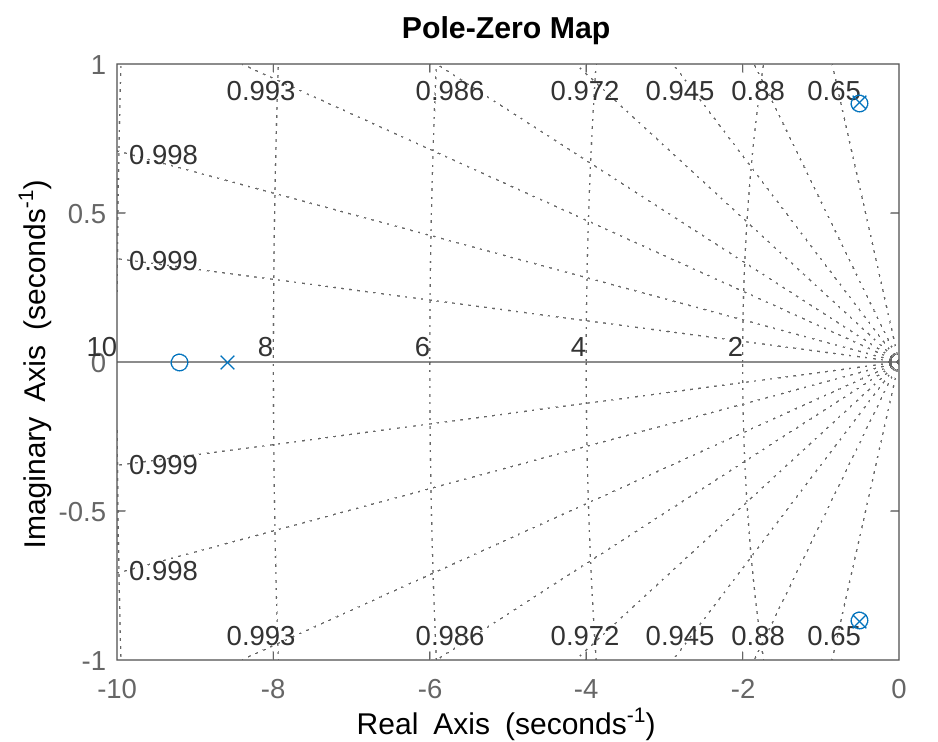
\includegraphics[scale=0.4]{Problem2Fig1.png}\\
As we can see, the poles all have their real parts less than 0, which means the system is stable.
\section*{Problem 3}
The blockdiagram for the nonlinear system looks like the following\\
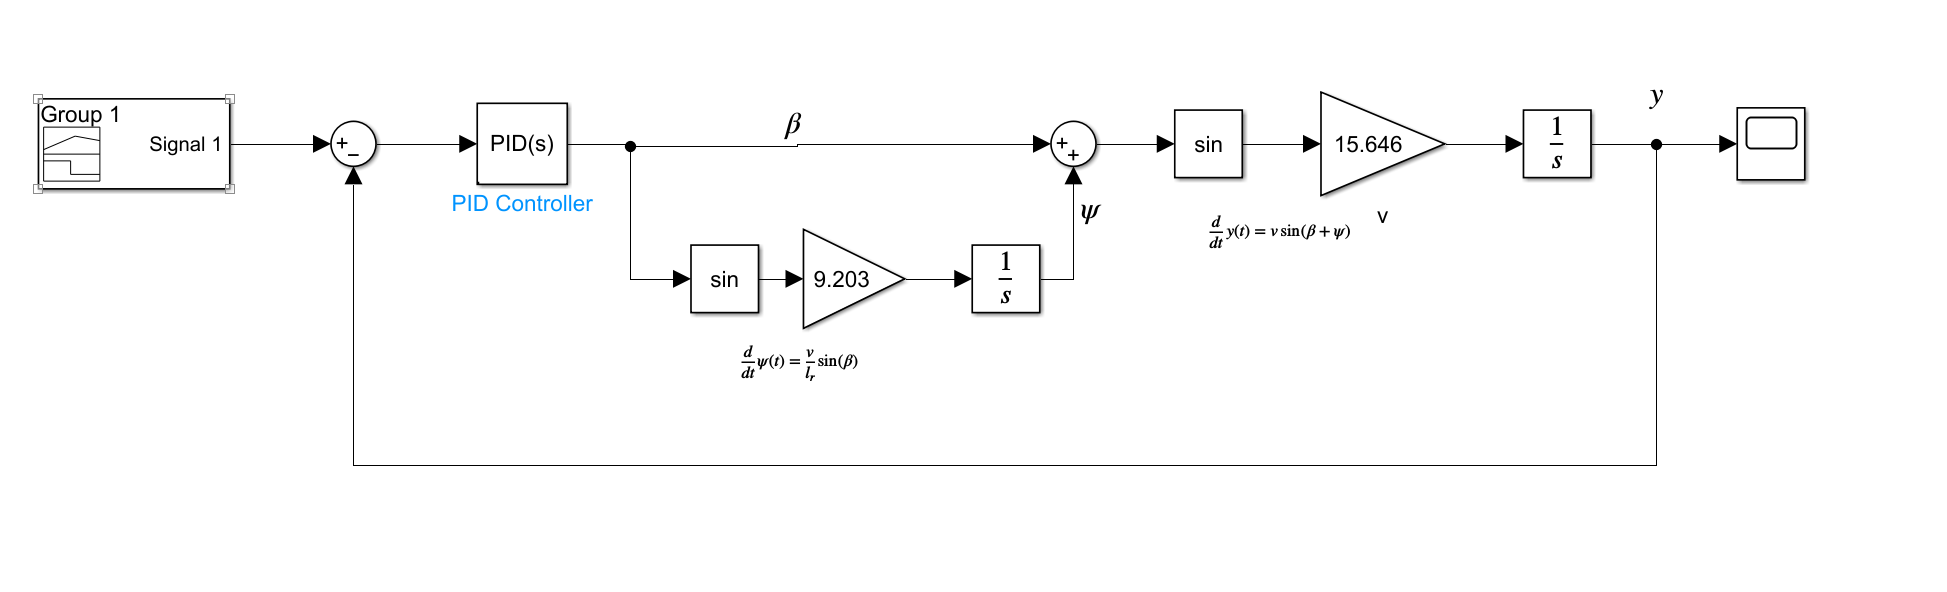
\includegraphics[scale=0.4]{Problem3BlockDiagram.PNG}\\
We can modify the inital conditions by modifying the inital conditions for the itegrator blocks. We define acceptable behaviour such that the absolute value of $y$ is less than
$\frac{3.0-1.8}{2}=0.6$, ie the car cannot move out of its own lane
\\\\
Using the following matlab code we can plot out where the initial values of $y$ and $\psi$ result in acceptable behaviour
\begin{verbatim}
psi_sweep=0:0.25:2*pi;
y_sweep=-3:0.1:-1;
t_final=40;
valid = zeros(length(psi_sweep),length(y_sweep));
for i=1:length(psi_sweep)
    psi_initial=psi_sweep(i);
    for j=1:length(y_sweep)
        y_initial=10^(y_sweep(j));
        a=sim("Problem3.slx");

        data=a.yout.getElement("y");
        
        if max(abs(data.Values.Data))<0.6
            valid(i,j)=1;
        end
    end

end

imagesc(y_sweep,psi_sweep,valid)
colorbar
ylabel("\psi initial values")
xlabel("log(abs(y)) initial values")
\end{verbatim}
which outputs the following plot\\
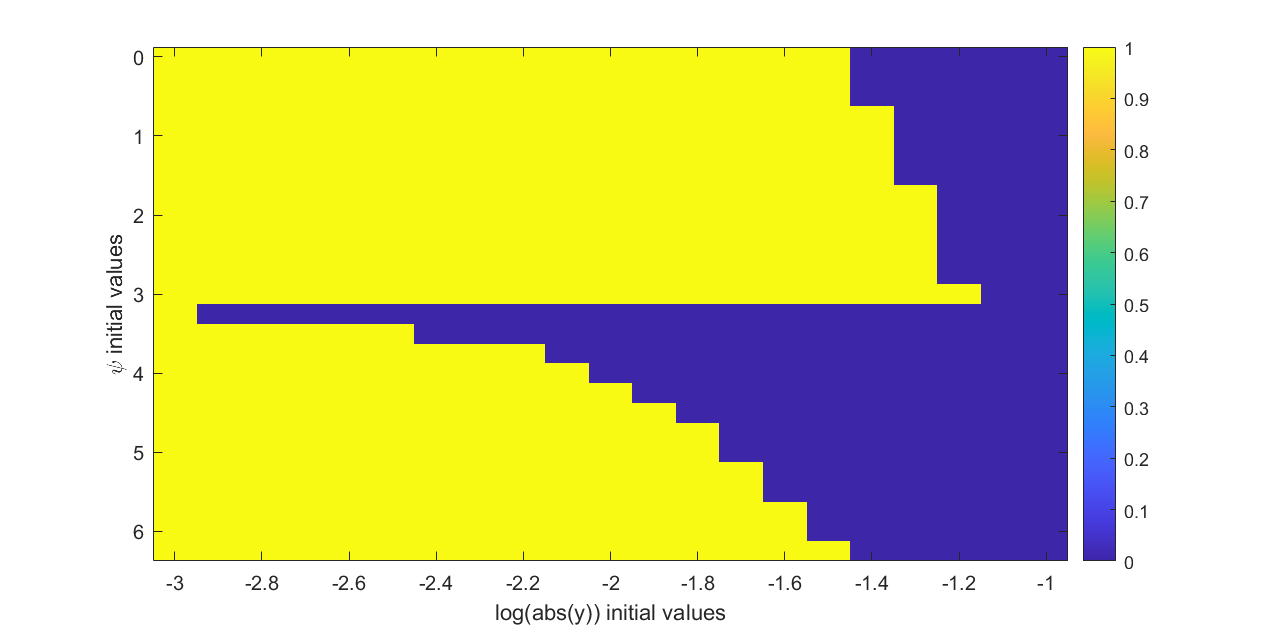
\includegraphics[scale=0.4]{Problem3Fig1.png}\\
Where the yellow block is the acceptable region, and the blue blocks are the unacceptable regions.\\
To check this, let us plot out the behaviour of the system for the initial conditions $y(0)=10^{-1.8}=0.0158$ and $\psi(0)=5$\\
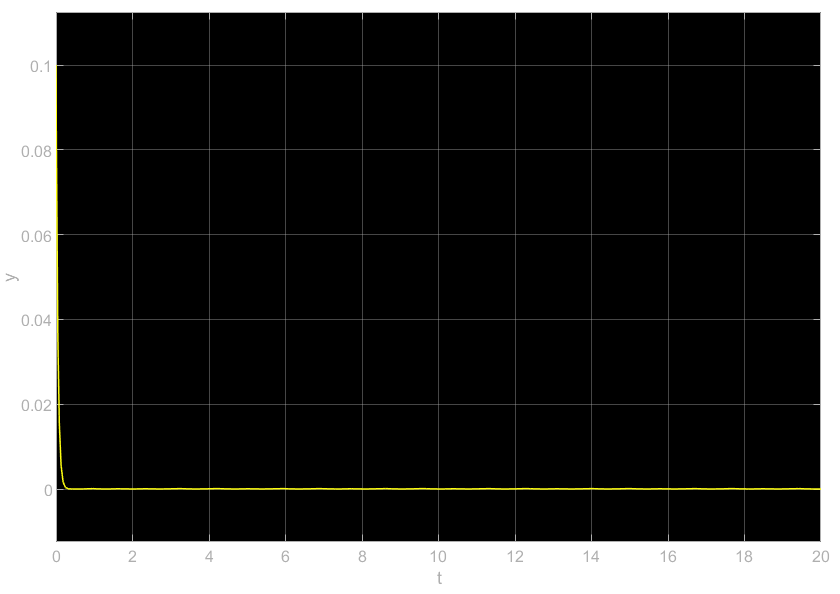
\includegraphics[scale=0.4]{Problem3Fig2.png}\\
As we can see, for these initial conditions, the maximum deviation is around $-0.1$ so the controller has adequate performance. Let us also plot out the car's y postion when
$y(0)=10^{-1.2}=0.0631$ and $\psi(0)=\frac{7\pi}{4}$,
\\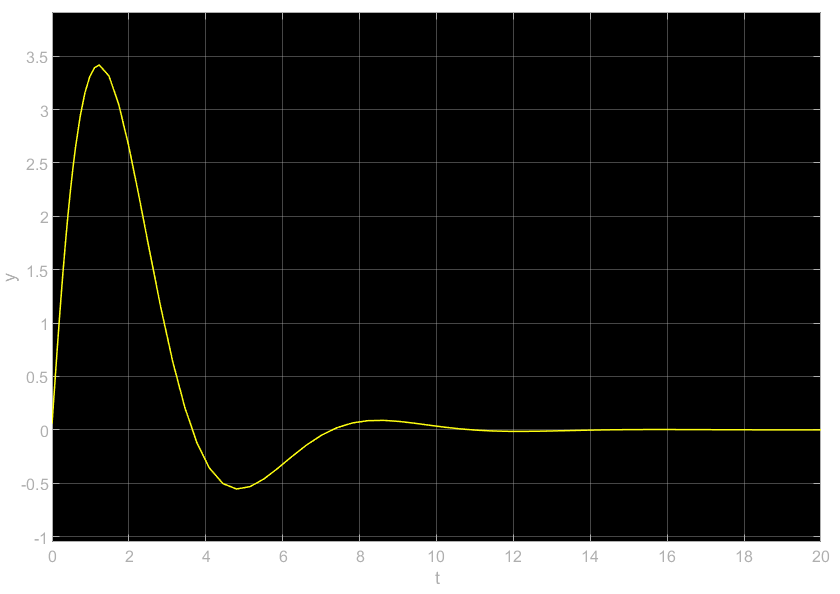
\includegraphics[scale=0.4]{Problem3Fig3.png}\\
As we can see for these intial conditions, the maximum deviation is around $3.5$ so the controller has inadequate performance for these inital conditions. Both of these discovers agree with the plot of initial conditions
that result in adequate performance that we generated
\section*{Problem 4}
We have
$$\frac{d}{dt}v=a$$
$$sv=a$$
$$\frac{v}{a}=\frac{1}{s}$$
therefore with a pid controller the transfer function from the input target velocity to the output velocity is 
$$\frac{(k_p+k_ds+k_i\frac{1}{s})\frac{1}{s}}{1+(k_p+k_ds+k_i\frac{1}{s})\frac{1}{s}}$$
Therefore the characteristic polyomial is 
$$s^2+(k_ps+k_ds^2+k_i)=0$$, therefore picking $k_p=k_i=k_d=1$ we get the following routh array from this matlab code
\begin{verbatim}
syms EPS;
k_d=1;
k_p=1;
k_i=1;
ra=routh([1+k_d k_p k_i],EPS)
\end{verbatim}
$$\begin{matrix}
    2 & 1\\
    1 & 0\\
    1 & 0\\
\end{matrix}$$
Therefore this controller stabilizes the system, to double check let us use the following matlab code to plot the poles and zeros of the transfer function
\begin{verbatim}
k_d=1;
k_p=1;
k_i=1;
sys = tf([k_d k_p k_i], [1+k_d k_p k_i]);
h = pzplot(sys);
grid on
\end{verbatim}
which outputs the following pole zero plot\\
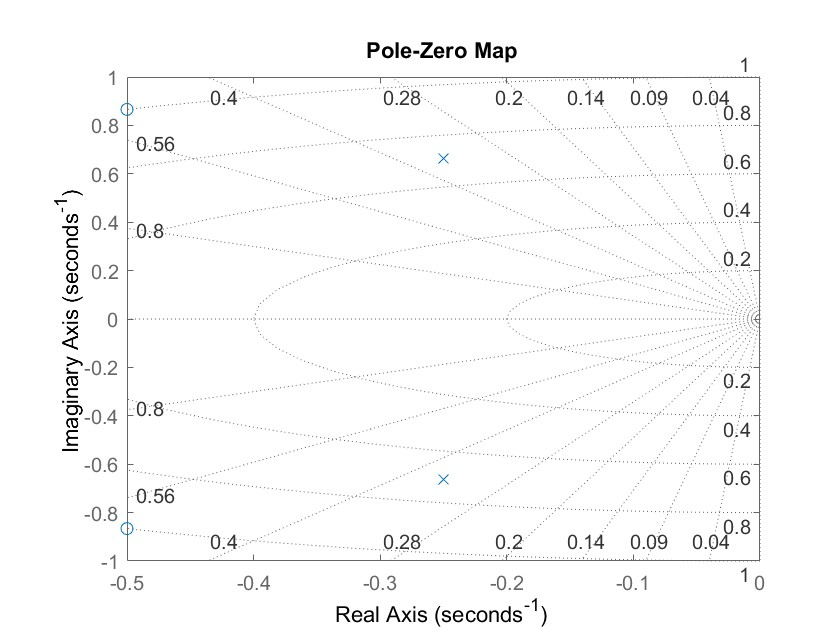
\includegraphics[scale=0.4]{Problem4Fig1.jpg}\\
\section*{Problem 5}
The blockdiagram for the nonlinear system looks like the following\\
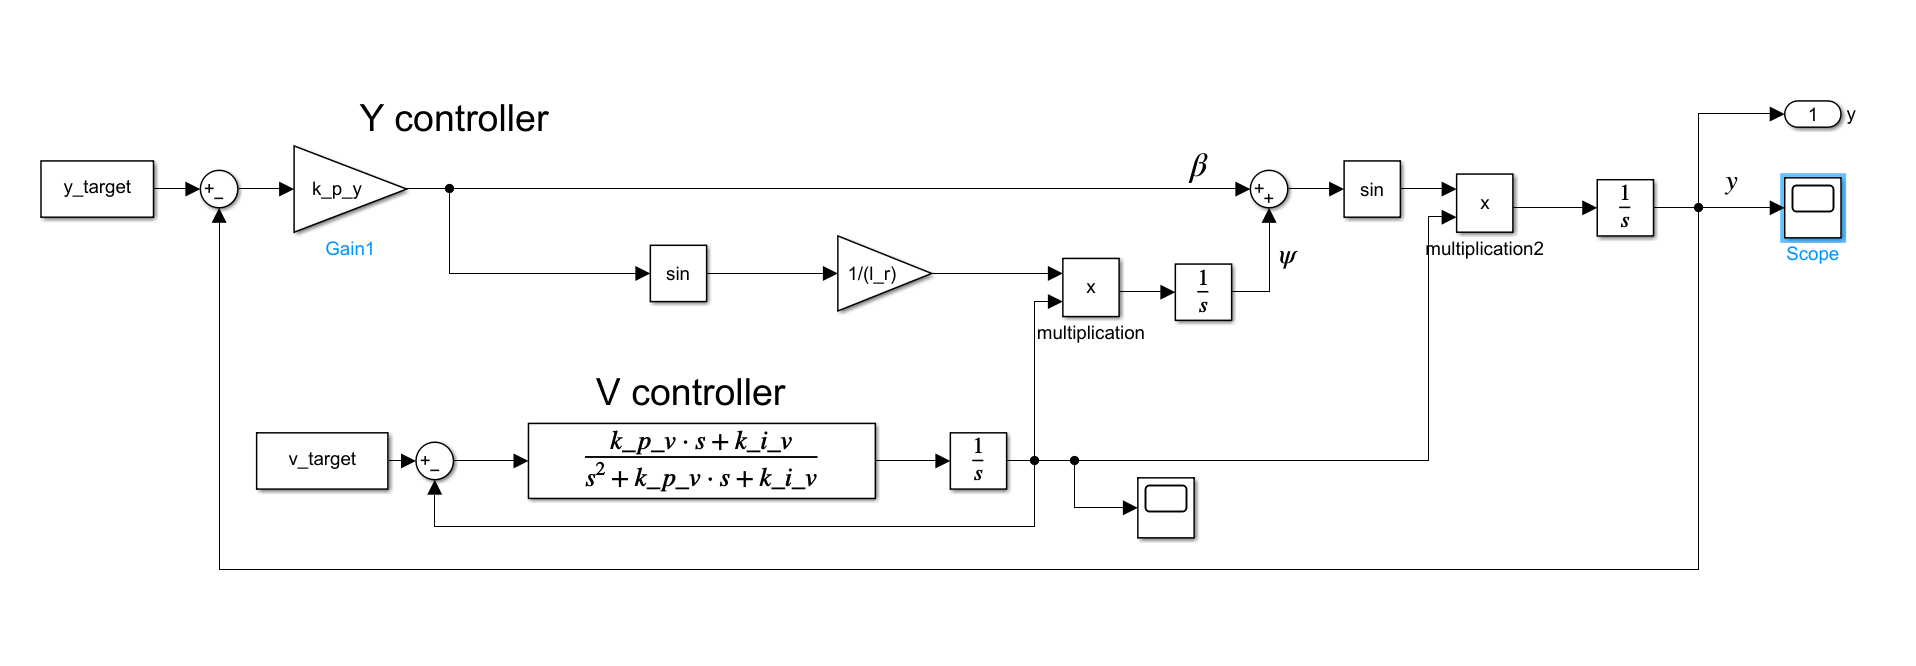
\includegraphics[scale=0.4]{Problem5BlockDiagram.PNG}\\

\end{document}